                                              \chapter{Motivation}

\section{Pourquoi l'algèbre linéaire ?}
Simplement par un plaisir sadique des responsables de l'éducation à l'EPFL... ?

Dommage, non. L'exemple classique d'une application de l'algèbre linéaire en informatique et communications est le machine learning, de plusieurs façons. Par exemple, la méthode de réduction de la dimensionnalité dite de \textit{l'analyse en composantes principales} a pour effet de réduire le nombre de paramètres régissant un certain ensemble de données en ne conservant que les principaux. La théorie se base en partie sur celle de \textit{la diagonalisation des endomorphismes linéaires}, dont vous traiterez en algèbre linéaire.
\begin{center}
    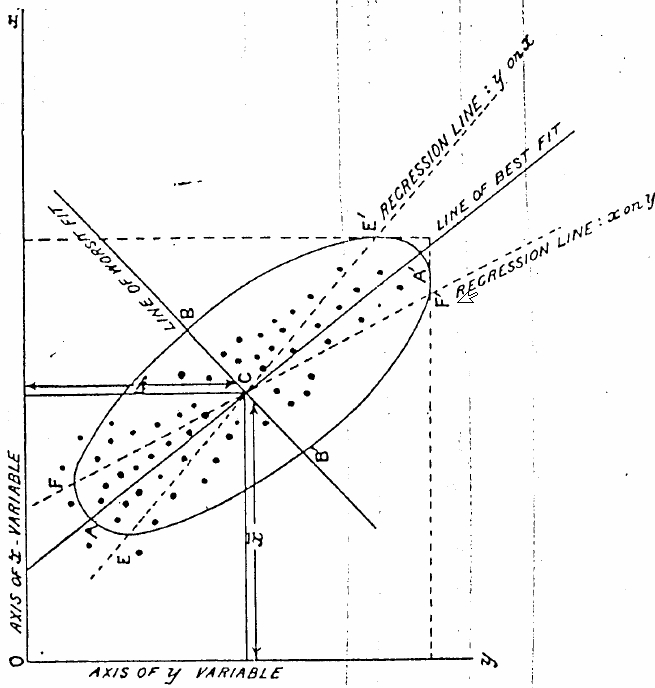
\includegraphics[width=9cm, height=8cm]{pearson}\\
    Wikimedia Commons: Karl Pearson, line of best fit diagram from Philosophical Magazine, 1901.
\end{center}
L'analyse en composantes principales a ses utilités hors du contexte du machine learning, en traitement du signal par exemple où \textit{la méthode des moindres carrés} permet de décomposer toute fonction périodique en une somme de $\cos$ et de $\sin$ plus faciles à traiter. Ceci permettra par exemple \textit{d'échantilloner} un signal continu tel qu'un son pour lui appliquer des traitements avant de le reconstituer. Dès votre premier semestre, en cours d'algèbre linéaire, il est possible que vous traitiez de la \textit{régression linéaire} comme application directe de la méthode des moindres carrés qui y sera présentée. De façon plus générale, l'algèbre linéaire est omniprésente dans le monde scientifique car les matrices permettent de représenter des données quelconques et de les manipuler très facilement.

\noindent Ici, bien entendu, nous n'avons même pas égratigné l'iceberg des applications de l'algèbre linéaire, nous pourrions y passer des heures.

\section{Qu'est-ce que l'algèbre linéaire ?}
C'est, pragmatiquement, une branche des mathématiques très bien comprise, dans le sens : mieux comprise que nombre d'autres qui réservent davantage de mystères et hypothèses pas encore prouvées. On y étudie comment généraliser l'intuition géométrique acquise dans la géométrie planaire et la géométrie dans l'espace, et ce que cette généralisation apporte.\\

\noindent Ce cours introductif, comme le cours d'Algèbre Linéaire de l'EPFL, fera les hypothèses les plus minimes possibles sur vos apprentissages précédents de la matière. Ainsi, nous ne supposerons \textit{pas} que vous savez ce qu'est une matrice, encore moins un espace vectoriel, et nous repartons de zéro dès la section suivante.\\